\begin{frame}{Статистика доказательств с использованием контекста}
\centering

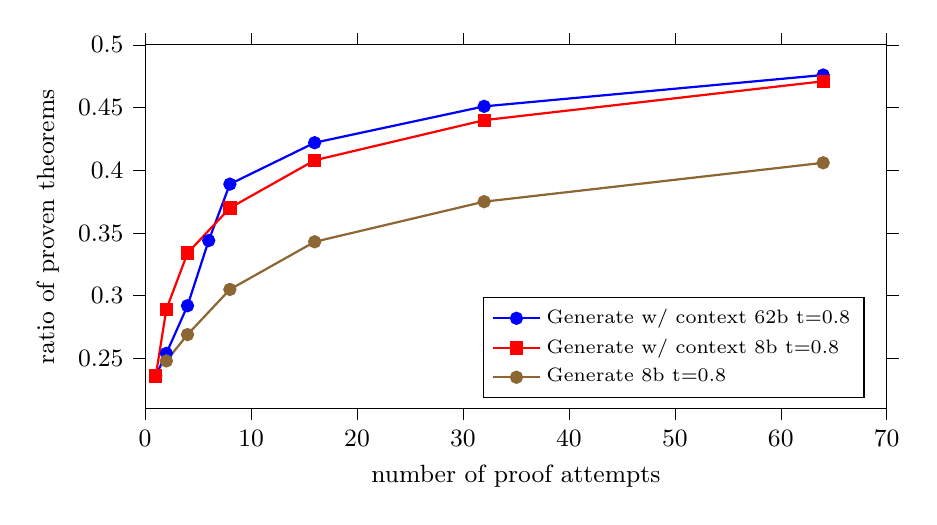
\begin{tikzpicture}
\begin{axis}[
    width=11cm,
    height=6.2cm,
    xmin=0, xmax=70,
    ymin=0.21, ymax=0.50,
    xlabel={number of proof attempts},
    ylabel={ratio of proven theorems},
    xtick={0,10,20,30,40,50,60,70},
    ytick={0.25,0.30,0.35,0.40,0.45,0.50},
    tick align=outside,
    axis line style={black},
    tick style={black},
    label style={font=\small},
    tick label style={font=\small},
    legend style={
        at={(0.97,0.03)},
        anchor=south east,
        draw=black,
        fill=white,
        font=\scriptsize,
        legend cell align=left
    }
]

% Generate w/ context 62b t=0.8
\addplot[
    color=blue,
    mark=*,
    thick
] coordinates {
    (1,0.236)
    (2,0.254)
    (4,0.292)
    (6,0.344)
    (8,0.389)
    (16,0.422)
    (32,0.451)
    (64,0.476)
};
\addlegendentry{Generate w/ context 62b t=0.8}

% Generate w/ context 8b t=0.8
\addplot[
    color=red,
    mark=square*,
    thick
] coordinates {
    (1,0.236)
    (2,0.289)
    (4,0.334)
    (8,0.370)
    (16,0.408)
    (32,0.440)
    (64,0.471)
};
\addlegendentry{Generate w/ context 8b t=0.8}

% Generate 8b t=0.8
\addplot[
    color={rgb,1:red,0.55;green,0.40;blue,0.20},
    mark=*,
    thick
] coordinates {
    (2,0.248)
    (4,0.269)
    (8,0.305)
    (16,0.343)
    (32,0.375)
    (64,0.406)
};
\addlegendentry{Generate 8b t=0.8}

\end{axis}
\end{tikzpicture}

\vspace{0.2cm}
{\small Ratio of theorems proven vs.\ inference cost for models with different sizes and temperatures.}
\end{frame}